\documentclass[11p]{article}
% Packages
\usepackage{amsmath}
\usepackage{graphicx}
\usepackage[swedish]{babel}
\usepackage[
    backend=biber,
    style=authoryear-ibid,
    sorting=ynt
]{biblatex}
\usepackage[utf8]{inputenc}
\usepackage[T1]{fontenc}
%Källor
\addbibresource{mall.bib}
\graphicspath{ {./images/} }

\title{Labrapprt \\ \small Fysik 1}
\author{Magnus Silverdal }
\date{\today}

\begin{document}

    \begin{titlepage}
        \begin{center}
            \vspace*{1cm}

            \Huge
            \textbf{Laboration 5}

            \vspace{0.5cm}
            \LARGE
            Ellära

            \vspace{1.5cm}

            \textbf{Malte Lindkvist}

            \vfill


            Fysik 1

            \vspace{0.8cm}

            
\includegraphics[width=0.4\textwidth]{../images/NTI Gymnasiet_Symbol_print_svart.png}

            \Large
            Teknikprogrammet\\
            NTI Gymnasiet\\
            Umeå\\
            \today

        \end{center}
    \end{titlepage}
    \section{Del 1}
    Uppgiften var att koppla en krets genom en resistans, mäta strömmen och spänningen sedan räkna ut resistansens motstånd i Ohmslag.
    \subsection{Material och metod}
    Materialet vi använda oss av var två sladdar, 9V batteri, kopplingsutrustning och ett motstånd.

    \subsection{Resultat}
    Vi kopplade ihop sladdarna och resistansen enligt instruktionerna.
    Efter mätning kom vi fram till att spänningen var 7.8 V och att strömmen var 0.07 A
    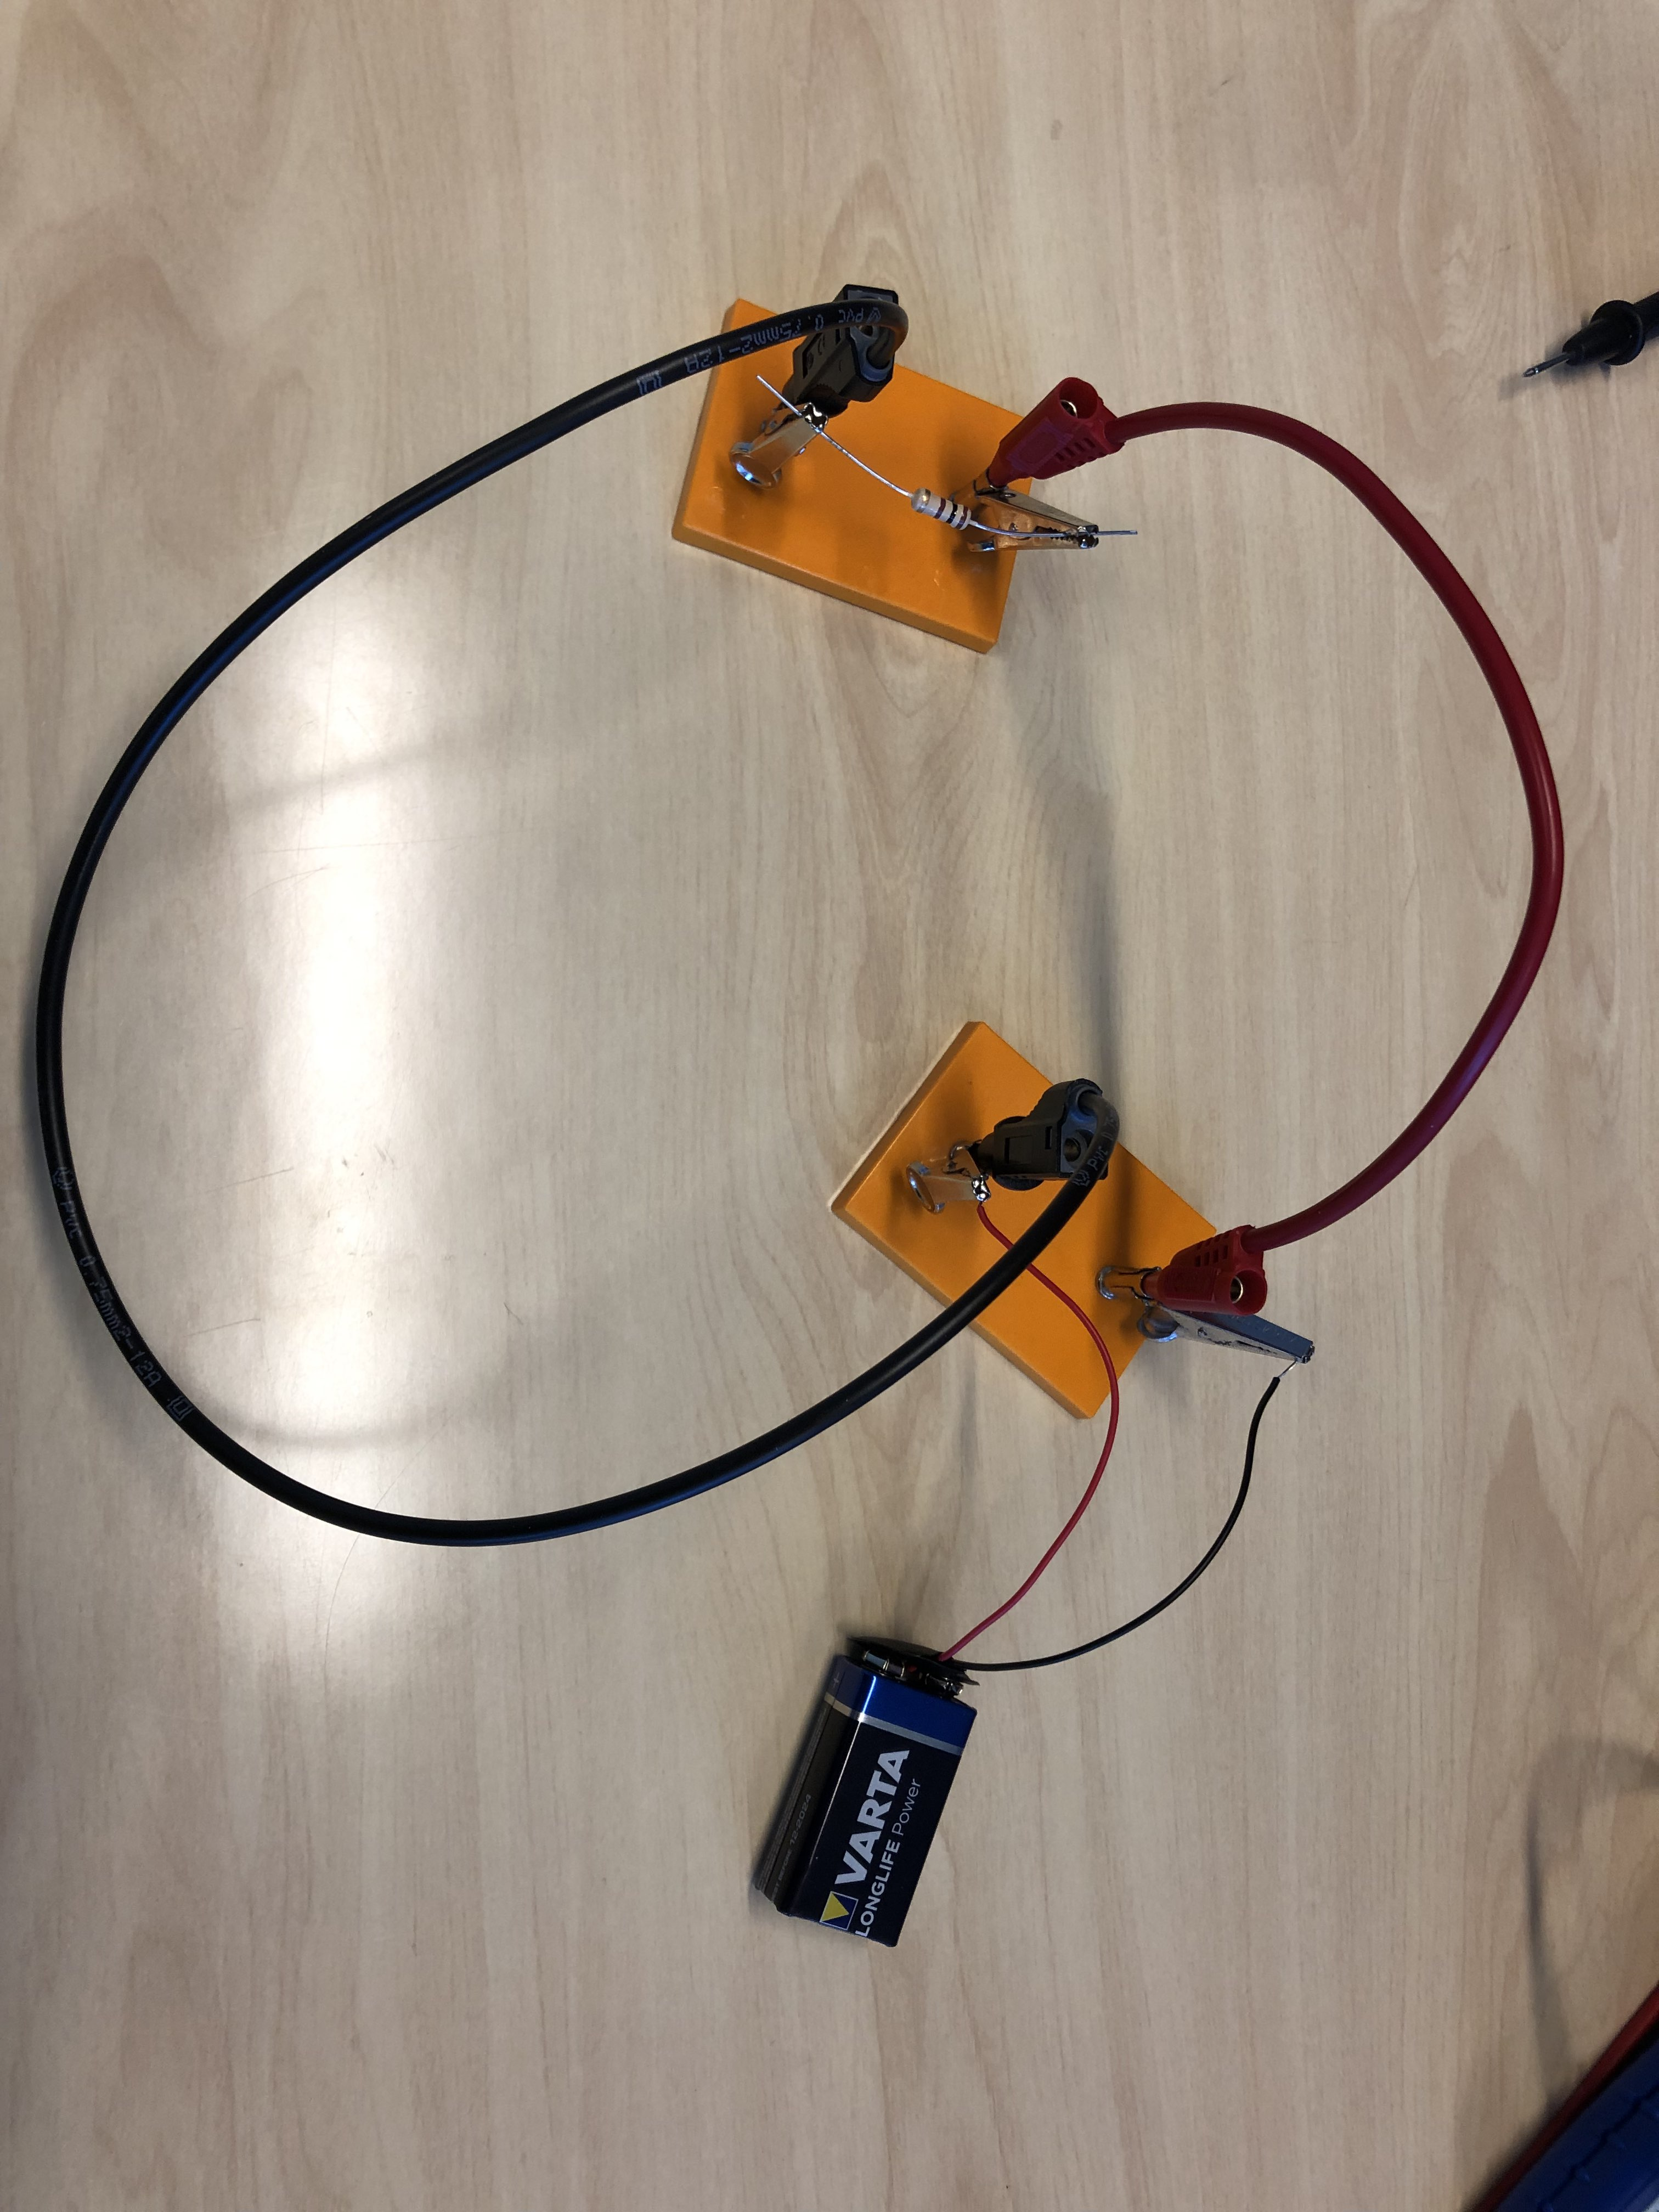
\includegraphics[width=0.4\textwidth]{../images/LabbDel1.jpg}

    Bilden ovan är den ihopkopplade kretsen på del 1
    \subsection{Analys}
    Med hjälp av formeln $ R=\frac{U}{I}$ kan vi räkna ut resistansen genom att ta $\frac{7.8}{0.07}=111$ Ohm
    \section{Del 2}
    Uppgiften var att mäta värdena på strömmen och spänningen sedan jämför värdena som vi teoretiskt borde fått fram och de som vi faktiskt fick fram.
    \subsection{Material och metod}
    Vi använde oss av 3 sladdar, 9V batteri, kopplingsutrustning och två motstånd.
    \subsection{Resultat}
    Vi kopplade ihop allting enligt vårat kopplingsschema.
    Efter att ha mätt spänning och strömmen kom vi fram till att U = 3.7V och I = 0.037A. Resistansen är $r=\frac{3.7}{0.037}=100$ Ohm

    \subsection{Analys}
    Ifall vi vill räkna ut det teoretiska värdena på spänningen och strömmen så antar vi att resistansen är 100 på grund av att det är ett bättre nummer än 111 och att det är den mer troliga resistansen (+att uträkningarna funkade inte riktigt ifall resistansen var 111 Ohm).
    9V går genom två motstånd som är seriekopplade, tillsammans blir de 200 Ohm av motstånd. Ifall vi använder oss av formeln $ R=\frac{U}{I}$
    och omvandlar den till $ I=\frac{U}{R}$ kan vi istället för att räkna ut resistansen räkna ut den teoretiska strömmen,
    den teoretiska strömmen blir då $ I=\frac{9}{200}=0.045 A $. Den teoretiska spänningen kommer bli 9V eftersom att batteriet är 9V
    och kretsen är seriekopplad kommer dessa 9V inte ta vägen någon stans (teoretiskst). Skillnaden i spänningen borde
    möjligtvis vara några volt på grund av inre resistans men att skillnaden är 5.3 volt verkar vara lite mycket, detta kan bero på fel uträkning (inte så sannolikt) eller fel
    mätvärden, det kan även bero på en dåligt fastsatt kabel. Skillnaden i ström kan bero på bero på inre resistans eller kabelförluster.

    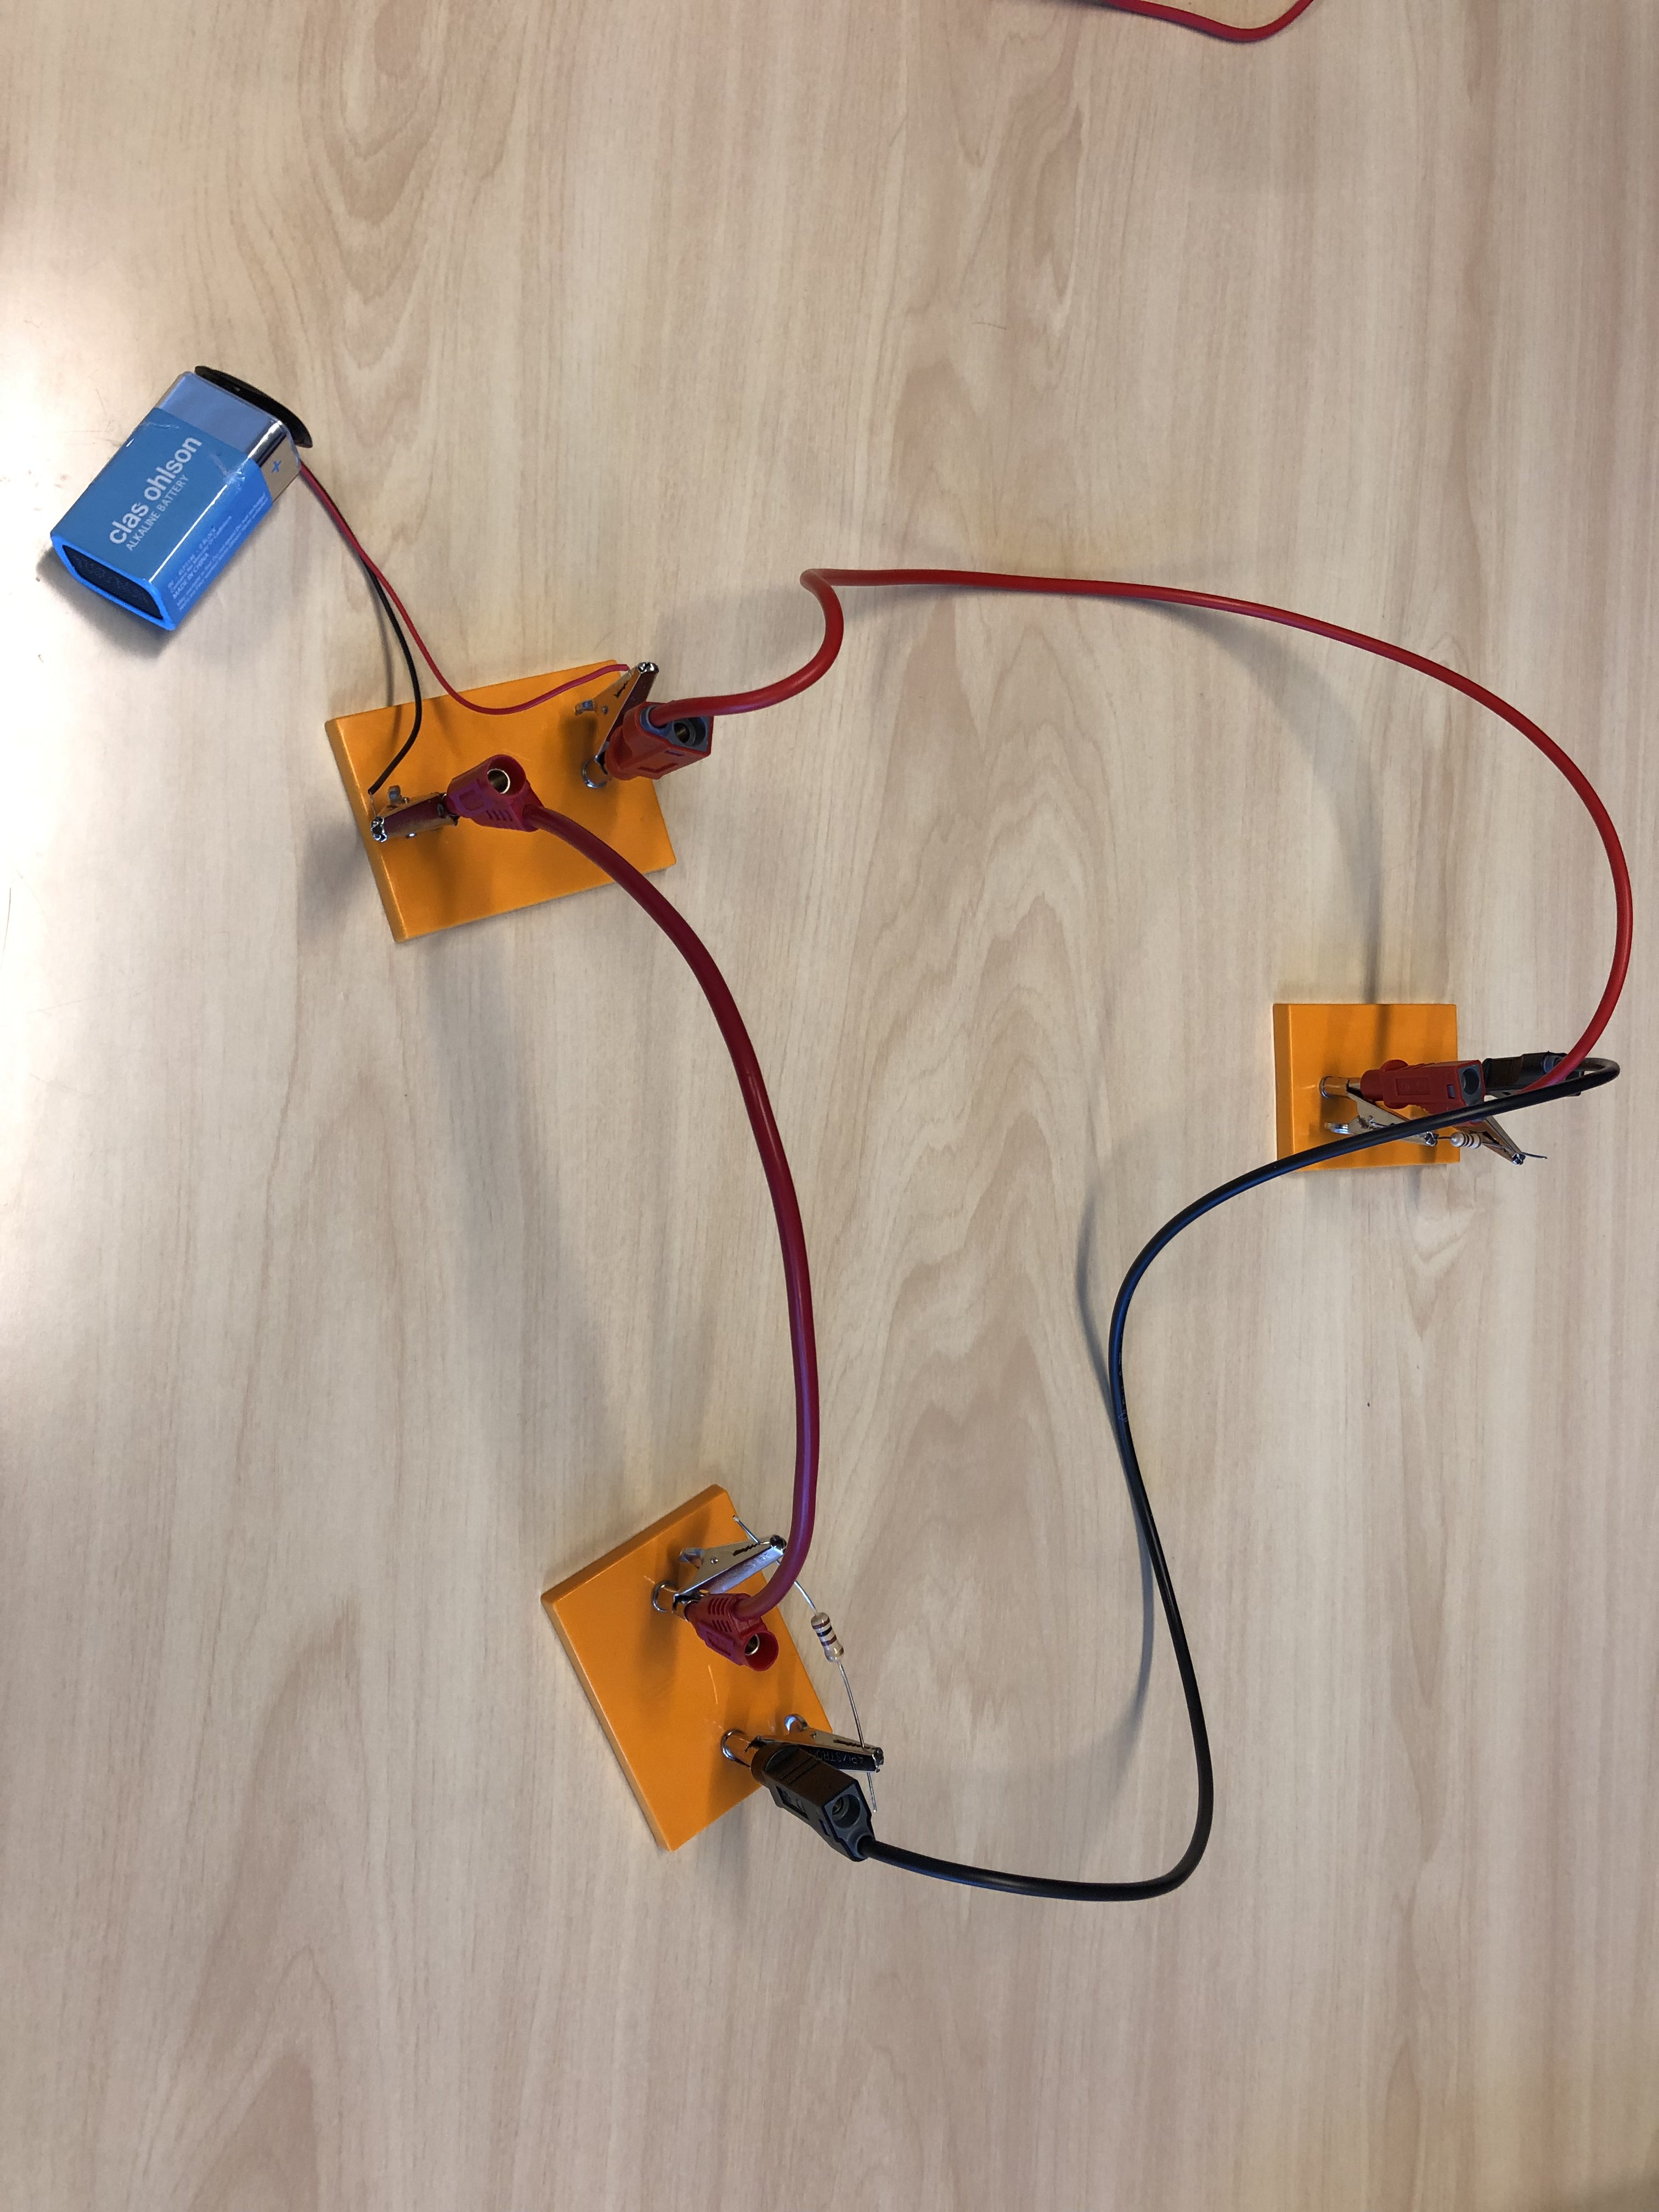
\includegraphics[width=0.4\textwidth]{../images/LabbDel2.jpg}

    Bilden ovan är den ihopkopplade kretsen på del 2
    \section{Del 3}
    I den tredje labben var uppgiften att parallelkoppla två motstånd med ett batteri, mäta värdena och sedan jämföra de värdena med de teoretiska värdena.
    \subsection{Material och metod}
    Vi använde oss av 4 sladdar, ett 9V batteri, kopplingsutrustning och två motstånd.
    \subsection{Resultat}
    Efter att vi parallelkopp   lade batteriet med två resistanser och mätt spänningen kom vi fram till att den var 6.6 V medans strömmen var 66mA eller 0.066 A.
    \subsection{Analys}
    Ifall vi vill räkna ut det teoretiska värdet igen kommer vi anta att resistansen är 100 Ohm, vi vet redan att batteriet är 9V, detta är allt som behövs för att räkna ut de teoretiska värdena.
    Vi behöver dock börja med att slå ihop de parallelkopplade resistanserna i en, detta görs med hjälp av formeln $\frac{1}{R} = \frac{1}{R1} + \frac{1}{R2}$. $\frac{1}{100}+\frac{1}{100}=\frac{2}{100}$ Sedan behöver man invertera värdena för att få fram resistansen, $\frac{100}{2}=50 Ohm$.
    Nu när vi lagt ihop båda resistanserna och tagit reda på att den totala resistansen är 50 Ohm kan vi använda detta i vår uträkning.
    Nu använder vi oss av formeln $I = \frac{U}{R} $, eftersom att spänningen kommer vara lika överallt borde den teoretisk vara 9V,
    $\frac{9}{50}=0.18 A $. Men eftersom att strömmen går genom två kretsar borde detta delas på två $\frac{0.18}{2}= 0.09 A $.
    Den teoretiska spänningen är alltså 9V och den teoretiska strömmen över en resistans är 0.09A, de faktiska värdena var
    0.066A och 6.6V, skillnaden beror antagligen på inre resistans och ett gammalt batteri.

    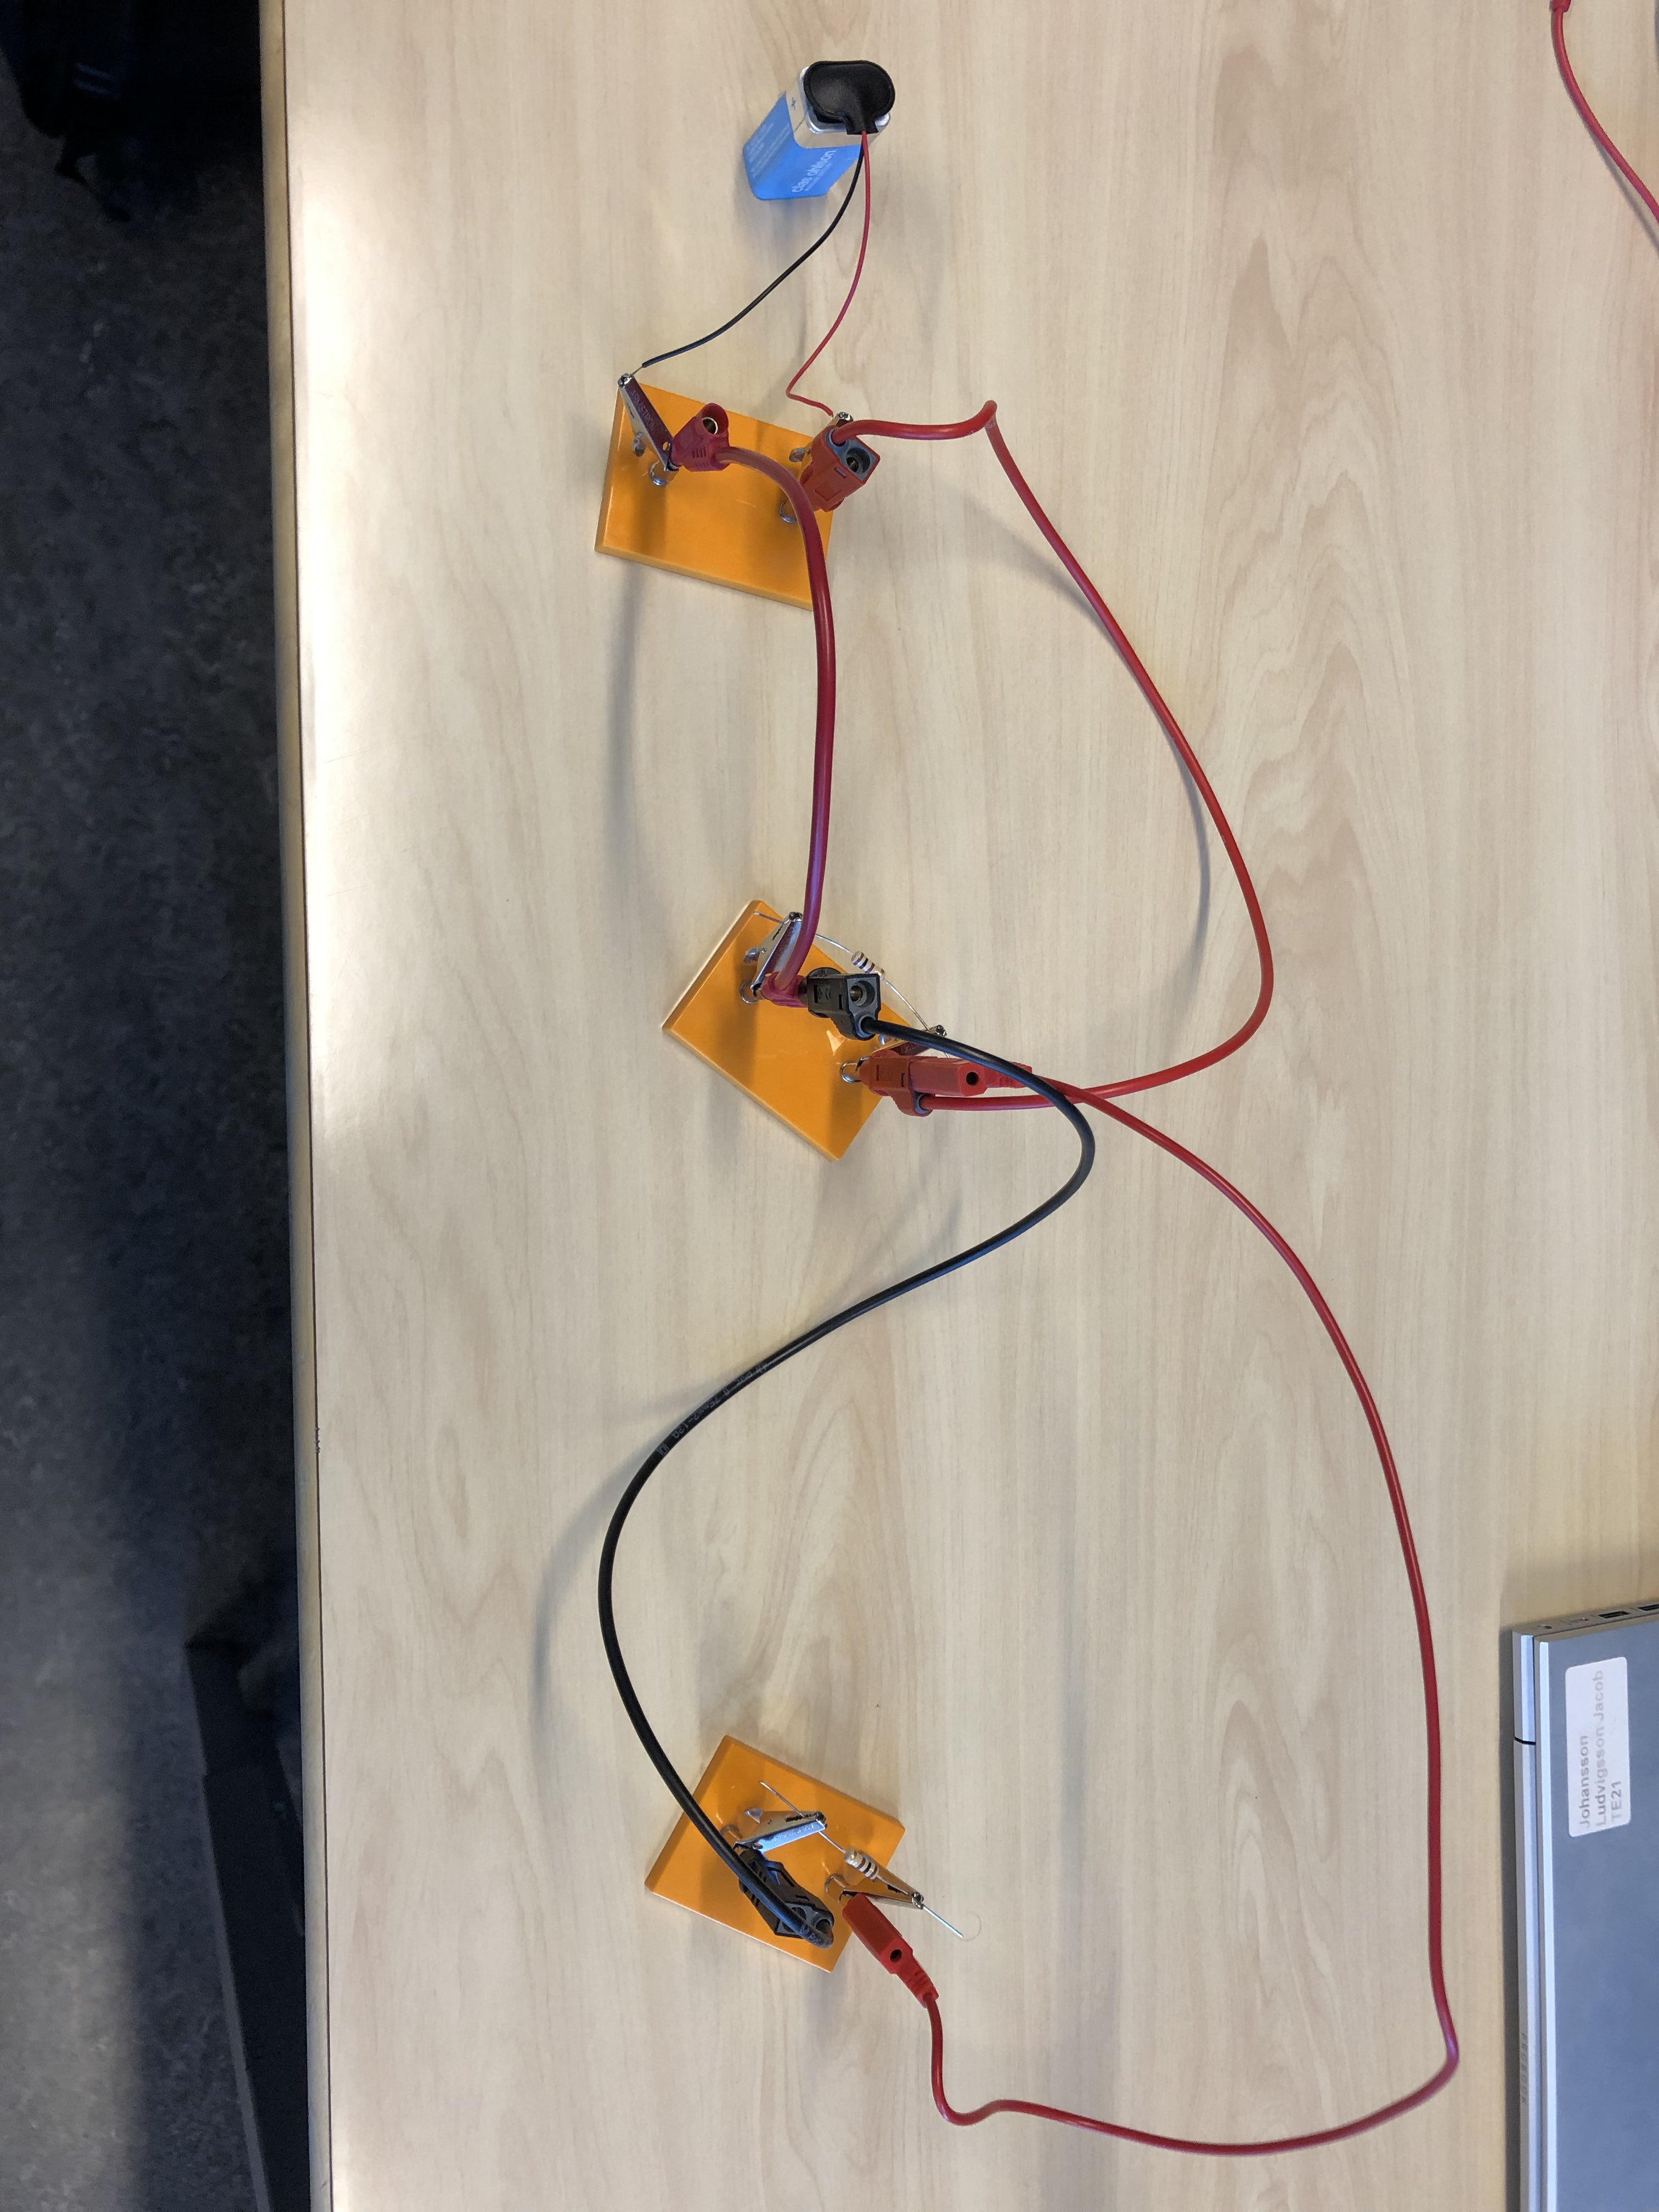
\includegraphics[width=0.4\textwidth]{../images/LabbDel3.jpg}

    Bilden ovan är den ihopkopplade kretsen på del 3
\end{document}
